\chapter{Performance des outils de détection }
\label{lab:chapCAD}
	\section{Généralités}

En oncologie, la détection des site tumoraux est une étape capitale dans la prise en charge des patients. Elle permet l'évaluation de l'état d'avancement de la maladie, ou encore d'étudier la réponse à un traitement~\cite{dimitrakopoulou2002role}. Cette détection se fait actuellement par le médecin qui va observer les images TEP/TDM acquises à la recherche de fixations anormales. Cependant, ces fixations peuvent provenir d'autres facteurs, tels que la ``graisse brune'', des muscles activés ou encore une inflammation locale~\cite{bordessoule2006impact}. Associés aux limites de l'imageur, surtout au niveau du rapport signal sur bruit des volumes reconstruits, il est donc possible qu'il y ait une erreur lors du diagnostique.

Dans cette partie, je vais détailler les techniques qui permettent de comparer les performances de plusieurs observateurs (médecins ou algorithmes) face aux mêmes images, ou alors du même observateur face à plusieurs types d'images différentes.

Pour l'instant le problème va être simplifié au cas où un observateur doit classer un signal en ``Sain'' (normal, HO) ou ``Pathologique'' (anormal, H1).
Les performances d'un classifieur sont indiquées par la matrice de confusion (table~\ref{tab:confusion}), qui recense les signaux correctement et incorrectement classés 

\begin{table}[h]
	\label{tab:confusion}
	\begin{tabular}{cc c|c|}
		& & \multicolumn{2}{c}{Classe estimée} \\
		\cline{3-4}	
		& & \multicolumn{1}{|c|}{Sain} & pathologique \\ 
		\cline{2-4}
		\multicolumn{1}{c|}{\multirow{2}{*}{Classe réelle}} & \multicolumn{1}{|c|}{Sain} & VN (\emph{Vrai Négatif}) & FP (\emph{Faux Positif})\\
		\cline{2-4}
		\multicolumn{1}{c|}{} & \multicolumn{1}{|c|}{Pathologique} & FN (\emph{Faux Négatif}) & VP (\emph{Vrai Positif})\\
		\cline{2-4}
	\end{tabular}
	\caption{Matrice de confusion : donne une vue d'ensemble des performances du classifieur. Elle indique le résultat de la classification de signaux connus.}
\end{table}

On utilise habituellement deux grandeurs pour mesurer les performances d'un classifieur :

La \emph{sensibilité} (eq. \ref{eq:sensib}) correspond à la proportion d'images correctement évaluées pathologiques par l'observateur par rapport au nombre total d'images réellement pathologiques. Elle donne une information sur la capacité du classifieur à détecter les cas pathologiques.

\begin{equation}
	\label{eq:sensib}
	Sensibilite = \frac{VP}{VP + FN}
\end{equation}

La \emph{spécificité} (eq. \ref{eq:specif}) représente le même type de grandeur, mais cette-fois ci appliquée aux cas non pathologiques : elle correspond à la capacité du test à donner un résultat négatif lorsque l'image est non pathologique.

\begin{equation}
	\label{eq:specif}
	Specificite = \frac{VN}{VN + FP}
\end{equation}

Ces deux grandeurs sont complémentaires mais ne permettent pas à elle seules de comparer des classifieurs. En effet, un  utilisateur va donner des notes, qui vont indiquer son degré de certitude sur la présence de la pathologie (à ne pas confondre avec des notations sur la gravité des lésions, comme les techniques de gradation de~\cite{genestie1998comparison}).

Les techniques de comparaisons d'organes de décision comme les ROC (Receiver-Operating Curve) permettent de prendre en compte ces incertitudes. Elles proviennent à l'origine du domaine des télécommunications pendant la seconde guerre mondial, où il fallait une métrique permettant de tester les performances des systèmes RADAR~\cite{zou2007receiver} pour la détection des avions ennemis. Les courbes ROC servent donc à évaluer la capacité de un ou plusieurs ``observateurs'' à discriminer des signaux entre deux classes ``normal'' et ``anormal''. Les informations de sensibilité et de spécificité se limitent à comparer les performances pour un niveau de détection donné.

	\section{Méthodologie ROC - Receiver-Operating Curve}

Les ROC \cite{swets1982evaluation}\cite{metz1986roc} sont des courbes indiquant la spécificité et la sensibilité du modèle de classification pour différents niveaux de certitudes. Elles fournissent une mesure objective des performances d'un observateur dans une tâche de discrimination entre deux classes. 

Elles peuvent être utilisée pour comparer les performances relatives de différents observateurs ou pour déterminer leurs paramètres optimaux 

l'évaluation d'un observateur par la méthode ROC implique de créer un jeu de données de données labellisé en deux classes : Normale (H0) et Pathologiques (H1). L'observateur va se voir présenter l'ensemble des images et devra les noter individuellement selon un barème défini à l'avance (par exemple 0: pas du tout pathologique, 1: potentiellement pathologique, 3:équivoque, 6: certainement pathologique). Par convention, plus la note (notée $\lambda$) sera élevée, plus l'observateur va considérer qu'il est en présence d'un cas pathologique. A l'inverse, une note basse va indiquer un cas présumé sain.

L'observateur peut être un humain ou un algorithme, et les notes peuvent être discrètes ou continues.

Le tracé de la courbe ROC se fait en reportant la sensibilité et la valeur "1-spécificité" du classifieur pour différents seuils. Par construction, la courbe va commencer au point $(0,0)$ (tous les points sont marqués négatifs) et se terminer au point de coordonnée $(1,1)$ (tous les points sont marqués positifs).


Le formalisme ROC considère que les distributions de probabilité des notes des cas H0 et H1 suivent une loi gaussienne (voir fig. \ref{fig:loiROC}). Ce modèle de décision suppose que l'ensemble des valeurs de $\lambda$ évaluées sur des cas H0 (sain) suit une distribution de probabilité $P(\lambda_0, \sigma_0)$ de valeur moyenne $\lambda_0$ et d'écart-type $\sigma_0$. De même, les valeurs de $\lambda$ évaluées sur des cas H1 (pathologiques), suivent une distribution de probabiilité $P(\lambda_1, \sigma_1)$. Le mécanisme de décision se base sur le choix d'une valeur de seuil $\lambda_s$ au-delà de laquelle les observations sont considérées comme pathologiques.

\begin{figure}[h]
	
	\label{fig:loiROC}
	\begin{center}
	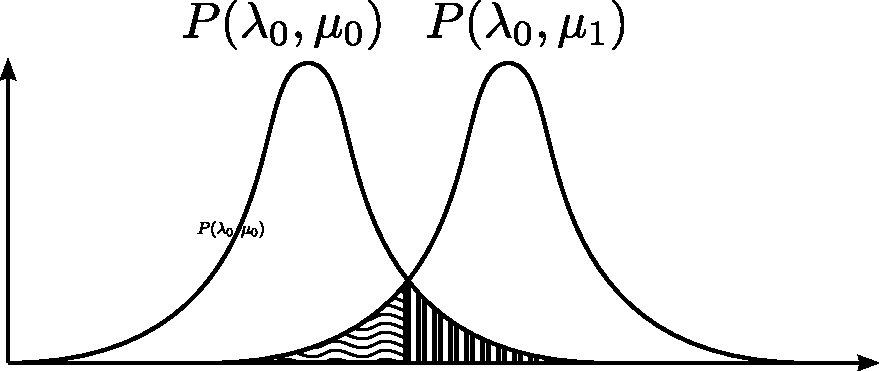
\includegraphics[width=10cm]{images/loiROC}
	\vspace{-0.5cm} % Ugly Moche Hideux
	\end{center}
	\caption{Modèle de la distribution de probabilité de la variable de décision dans pour les populations H0 ($P(\lambda_0, \mu_0)$) et H1 ($P(\lambda_1, \mu_1)$) dans les études ROC. $\lambda_s$ repésente le seuil à partir duquel une observation sera catégorisée H0 ou H1.}
\end{figure}

Ce seuil permet de modifier de manière dynamique la répartition des observations dans la matrice de confusion.  Cela permet d'enrichir la comparaison des observateurs par rapport au couple (sensibilité/spécificité) seul.


Un ensemble d'indicateurs permettent de comparer les performances de classifieurs à partir des courbes ROC. La performance est représentée par une FDM (Figure De Mérite). La FDM la plus simple consiste à choisir un niveau de spécificité (noté $\alpha$) et à comparer les sensibilités des différents classifieurs. L'avantage de ce système est qu'il permet de comparer les performances dans des conditions proches de la réalité, où l'on cherche à rester dans un taux de spécificité données. Cependant, les résultats vont dépendre du paramètre $\alpha$. Une métrique plus globale est l'aire sous la courbe ROC. \'Etant donné que la courbe sera nécessairement comprise dans un carré unitaire, la valeur de l'aire sera comprise entre 0 (le classifieur donne systématiquement les mauvaises réponses), 0.5 (le classifieur donne des réponses aléatoires) et 1 (le classifieur donne toujours la bonne réponse)\cite{nie2006integrating}.

IL est important lors du calcul de la FDM d'avoir une estimation de l'erreur. Il est possible de l'estimer en ajustant une courbe théorique (répondant à la loi théorique de la figure \ref{fig:loiROC}). Plusieurs logiciels ont été développés pour estimer les paramètres, qui ont été comparés dans la publication \cite{CarstenStephan03012003} (AccuROC, Analyse-It, CMDT, GraphROC, MedCalc, mROC, ROCKIT, and SPSS).

Une grandeur souvent utilisée dans la littérature pour évaluer la pertinence d'un résultat est la \emph{p-valeur}. Elle représente la probabilité d'obtenir un résultat au moins aussi extrème que le résultat obtenu (dans notre cas, la courbe ROC), en prenant en compte l'hypothèse selon laquelle le classifieur est aléatoire. Elle permet de vérifier si le test est statistiquement significatif.

Le problème des courbes ROC est que l'observateur ne donne pas d'information de localisation du problème dans l'image. Dans notre cas, nous voulons comparer des classifieurs qui détectent les tumeurs dans l'image. Il faut non seulement savoir si des lésions sont présentes, mais aussi avoir leur nombre et leur localisation. Cela est plus proche du travail en routine clinique qui consiste à évaluer l'étendue et le nombre des lésions pour déterminer l'efficacité d'un traitement par exemple. 

Pour éviter cette limitation, plusieurs extensions à la méthodologie \ROC sont décrites dans la littérature : L-ROC, AF-ROC ou encore F-ROC. Les L-ROC sont décrites ci-après, tandis que les AF-ROC et F-ROC seront décrites dans la section suivante.

\subsection{Courbes Localization ROC (L-ROC)}

L'analyse L-ROC~\cite{farquhar1999roc} ajoute l'information de localisation lors de la décision. L'observateur doit indiquer sur l'image qu'il considère comme pathologique la localisation de la lésion la plus probable. Elle est considérée comme un vrai positif si la distance entre la localisation indiquée et la localisation réelle de la lésion est inférieur à une certaine distance.

Cependant, bien que cette technique prenne en compte l'information de localisation, elle ne permet pas de traiter de manière satisfaisante les cas multi-lesions. 


\section{F-ROC}	


\subsection{Courbes Free-ROC}
\label{lab:FROC}

les courbes F-ROC~\cite{bunch1978free} sont une généralisation des courbes ROC aux cas où l'on évalue la capacité de l'observateur à détecter un ensemble de lésions dans une série d'images. Chaque image pouvant contenir un nombre indéfini de lésions. L'observateur va donc devoir pointer sur l'image l'ensemble des sites suspects et y associer une note.

Dans ce cas, on ne peut pas utiliser le formalisme ROC car le terme de spécificité n'est pas directement calculable pour chaque niveau de confiance. On utilise à sa place le nombre moyen de faux positifs par image pour un seuil donné (voir fig.\ref{fig:courbeFROC}).

On utilise les termes de LL (Localisation de Lésion) et NL (Non-Lésion) en lieu et place des informations de vrai positifs et faux positifs sur les courbes ROC. De la même manière, la sensibilité et la spécificité sont respectivement FLL (Fraction de localisation de lésion) et FNL (Fraction des Non-Lésions).

\begin{figure}[h]
	\label{fig:courbeFROC}
	\begin{center}
	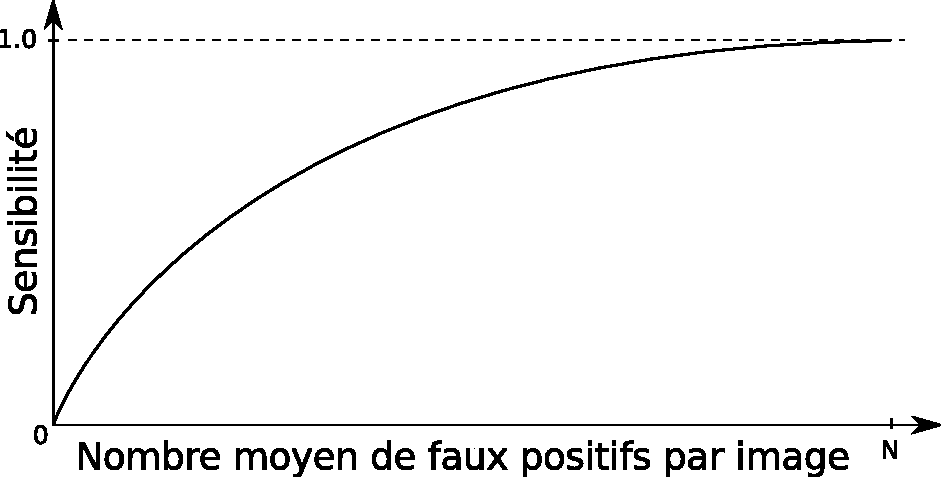
\includegraphics[width=15cm]{images/FROC}
	\end{center}
	\caption{Courbe Free ROC}
\end{figure}

Les courbes F-ROC n'ayant pas de bornes sur l'axes des abscisses, il est impossible de comparer plusieurs courbes à partir de l'aire sous la courbe. Il reste cependant possible de comparer la sensibilité pour un nombre de faux positifs donnés, mais on retrouve les mêmes problèmes que pour l'analyse ROC : il faut choisir un paramètre.

\subsection{Courbes Alternative Free-ROC}

Les courbes A-FROC~\cite{chakraborty1990free} sont des extensions des courbes Free-ROC présentées précédemment mais qui ne prennent en compte que le faux positif de plus haut score par image, ce qui ne pénalise pas le cas où un observateur indique un grand nombre de localisations sans lésions.

\subsection{Comparaison des courbes}
\label{lab:AFROC}
Plusieurs techniques ont été développées pour permettre de réaliser des comparaisons. De la même manière que pour les courbe ROC, il est possible de comparer les courbes F-ROC en fonction de la FLL pour un nombre de faux positifs donnés. Cependant, étant donné que les courbes F-ROC n'ont pas de fin déterminée, il n'est pas possible d'utiliser l'aire sous la courbe. JAFROC\cite{chakraborty2004observer} (JAcknife Free Receiver Operating Curve) est un algorithme et un logiciel développé par Chakraborty et se base sur une FDM non liée directement à la courbe. 

Cette mesure de performance utilise un algorithme dérivé des études A-FROC, ce qui signifie qu'il n'utilise pas l'ensemble des informations disponibles dans les courbes Free-ROC. Il va comparer les scores des faux positifs de plus forte note pour chaque image avec les notes des vrais positifs. La FDM mesure la probabilité d'avoir un score de vrai positif supérieur à celui d'un faux positif (de n'importe quelle image).

Soit $\theta$ la valeur de la FDM, $N_T$ le nombre total d'images, indexés par $i$, $N_A$ le nombre total de cas pathologiques, indexés par $j$. $n_j$ est le nombre total de lésions dans le cas anormal $j$.

\begin{equation}
\label{eq:JAFROC1}
\begin{array}{l}
	\displaystyle \theta=\frac{1}{N_T N_A} \sum_{i=1}^{N_T} \sum_{j=1}^{N_A} \sum_{k=1}^{n_j} W_{jk} \psi(X_i, Y_{jk}) \\
	\\
	\displaystyle \psi(X,Y) = \left\{
		\begin{array}{lll}
			1.0 & \mbox{si} & Y > X \\
			0.5 & \mbox{si} & Y = X    \\
			0.0 & \mbox{si} & Y < X    \\
		\end{array}
	\right. \\
	\\
	\displaystyle \mbox{avec} \sum_{k=1}^{n_j} W_{jk} = 1 \\
\end{array}
\end{equation}

$X_i$ le score du plus haut Faux positif de l'image $i$, $Y_{jk}$ est la note de la lésion k de l'image j. Si une lésion n'a pas été détectée, alors sa note sera par défaut de "0".

Les poids $W_{jk}$ correspondent à l'importance relative de détecter la lésion $k$ dans l'image $j$ pour le diagnostique. Pour chaque image, la somme des poids doit être égale à 1.

Une seconde version de JAfroc existe avec un pouvoir statistique plus important, mais elle nécessite de disposer d'un grand nombre de cas non pathologiques. La formule est la même que celle précédente (eq. \ref{eq:JAFROC1}). La seule différence est que la première sommation se fait sur l'ensemble des cas non pathologiques $N_N$ (eq. \ref{eq:JAFROC2}).

\begin{equation}
\label{eq:JAFROC2}
\theta=\frac{1}{N_T N_A} \sum_{i=1}^{N_N} \sum_{j=1}^{N_A} \sum_{k=1}^{n_j} W_{jk} \psi(X_i, Y_{jk})
\end{equation}


\chapter{Systèmes de détection}

	\section{Les CAD en TEP}

Les systèmes CAD (Computer-Aided-Detection) sont des algorithmes permettant d'assister le praticien dans la détection des lésions ou le classement des images images médicales. Dans le cadre de l'imagerie TEP oncologique, le besoin principal est celui du suivi thérapeutique. Pour cela, il est important de détecter d'éventuelles lésions résiduelles. Pour cela, il faut que le système CAD soit particulièrement adapté à la recherche de petites lésions de faible contraste qui pourraient échapper au médecin. Cependant, le diagnostique, qui consiste à évaluer la dangerosité des lésions, et leur caractère pathologique est une tâche plus complexe qui relève plus des système d'aide au diagnostique, qui ne seront pas traités ici.

Le développement des systèmes CAD a débuté dans les années 1980~\cite{chan1987image}, notamment pour détecter les micro calcifications en mammographie. Bien qu'il existe plusieurs systèmes CAD commerciaux pour l'imagerie TDM (xLNA pour philips par exemple), aucun CAD commercial pour la TEP n'existe à ma connaissance.

	\section{Types de classification}
		\subsection{supervisée - méthodologie}

Les classifieurs supervisés nécessitent une connaissance a priori des classes. On entraîne le classifieur en lui fournissant des \emph{exemples} de cas avec l'étiquette associée. A partir de cette base de données d'entraînement, le classifieur va générer un \emph{modèle} predictif permettant de classer de futurs exemples non encore connus.

\begin{figure}[h]
	\label{fig:fonctClassif}
	\begin{center}
	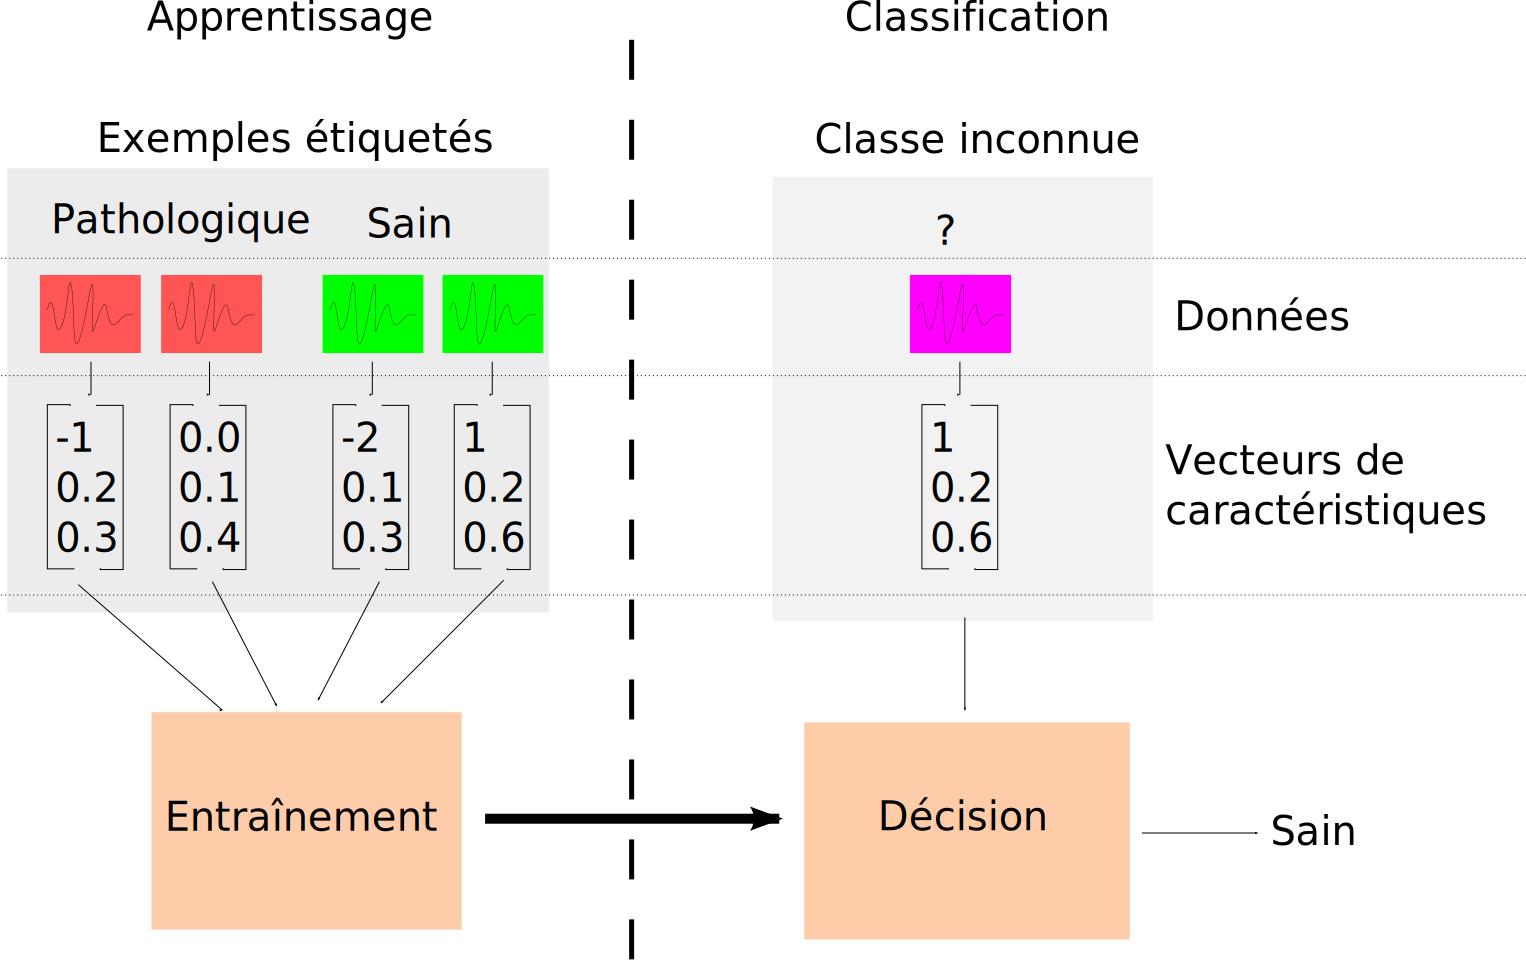
\includegraphics[width=15cm]{images/fonctionnementClassif}
	\end{center}
	\caption{Fonctionnement d'un classifieur supervisé : Les données d'apprentissage servent à entraîner le classifieur pour générer un modèle. Ce modèle permettra de rattacher des observations aux classes apprises.}
\end{figure}

		\subsubsection{Machines à vecteur de support (SVM)}
\label{lab:SVM}
La ``Machine à Vecteur de Support'', aussi appelée ``Séparateur à Vaste Marge'', ou ``Support Vector Machines'' en Anglais, est un classifieur qui comme son nom l'indique vise à maximiser la marge\cite{boser1992training}, qui est la distance entre les points des données et la surface spéaratrice (voir figure \ref{fig:SVM}).

\begin{figure}[h]
	\label{fig:SVM}
	\begin{center}
	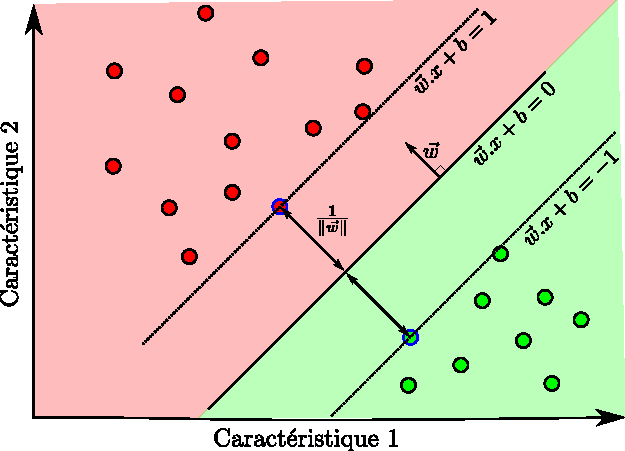
\includegraphics[width=12cm]{images/SVM}
	\end{center}
	\caption{Machine à Vecteur de Support : Les points vecteur de support (entourés de bleu) sont les seuls utilisés pour calculer la surface de séparation d'équation $\vec w . x + b = 0$. Le vecteur $\vec w$ est normal à la surface de séparation et permet de calculer la marge $\frac{1}{\Vert w \Vert}$.}
\end{figure}

		\subsection{non supervisée - méthodologie}

Dans le système de classification non supervisé, on fourni directement au classifieur l'ensemble des données à traiter. Il devra de lui-même les classer par similitude en groupes. On utilise ce type de classifieur si on ne connaît pas a priori les classes \ref{fig:fonctionnementClassifNonSup}.

La classification nom supervisée repose sur une méthode statistique utilisant une fonction de proximité.

\begin{figure}[h]
	\label{fig:fonctionnementClassifNonSup}
	\begin{center}
	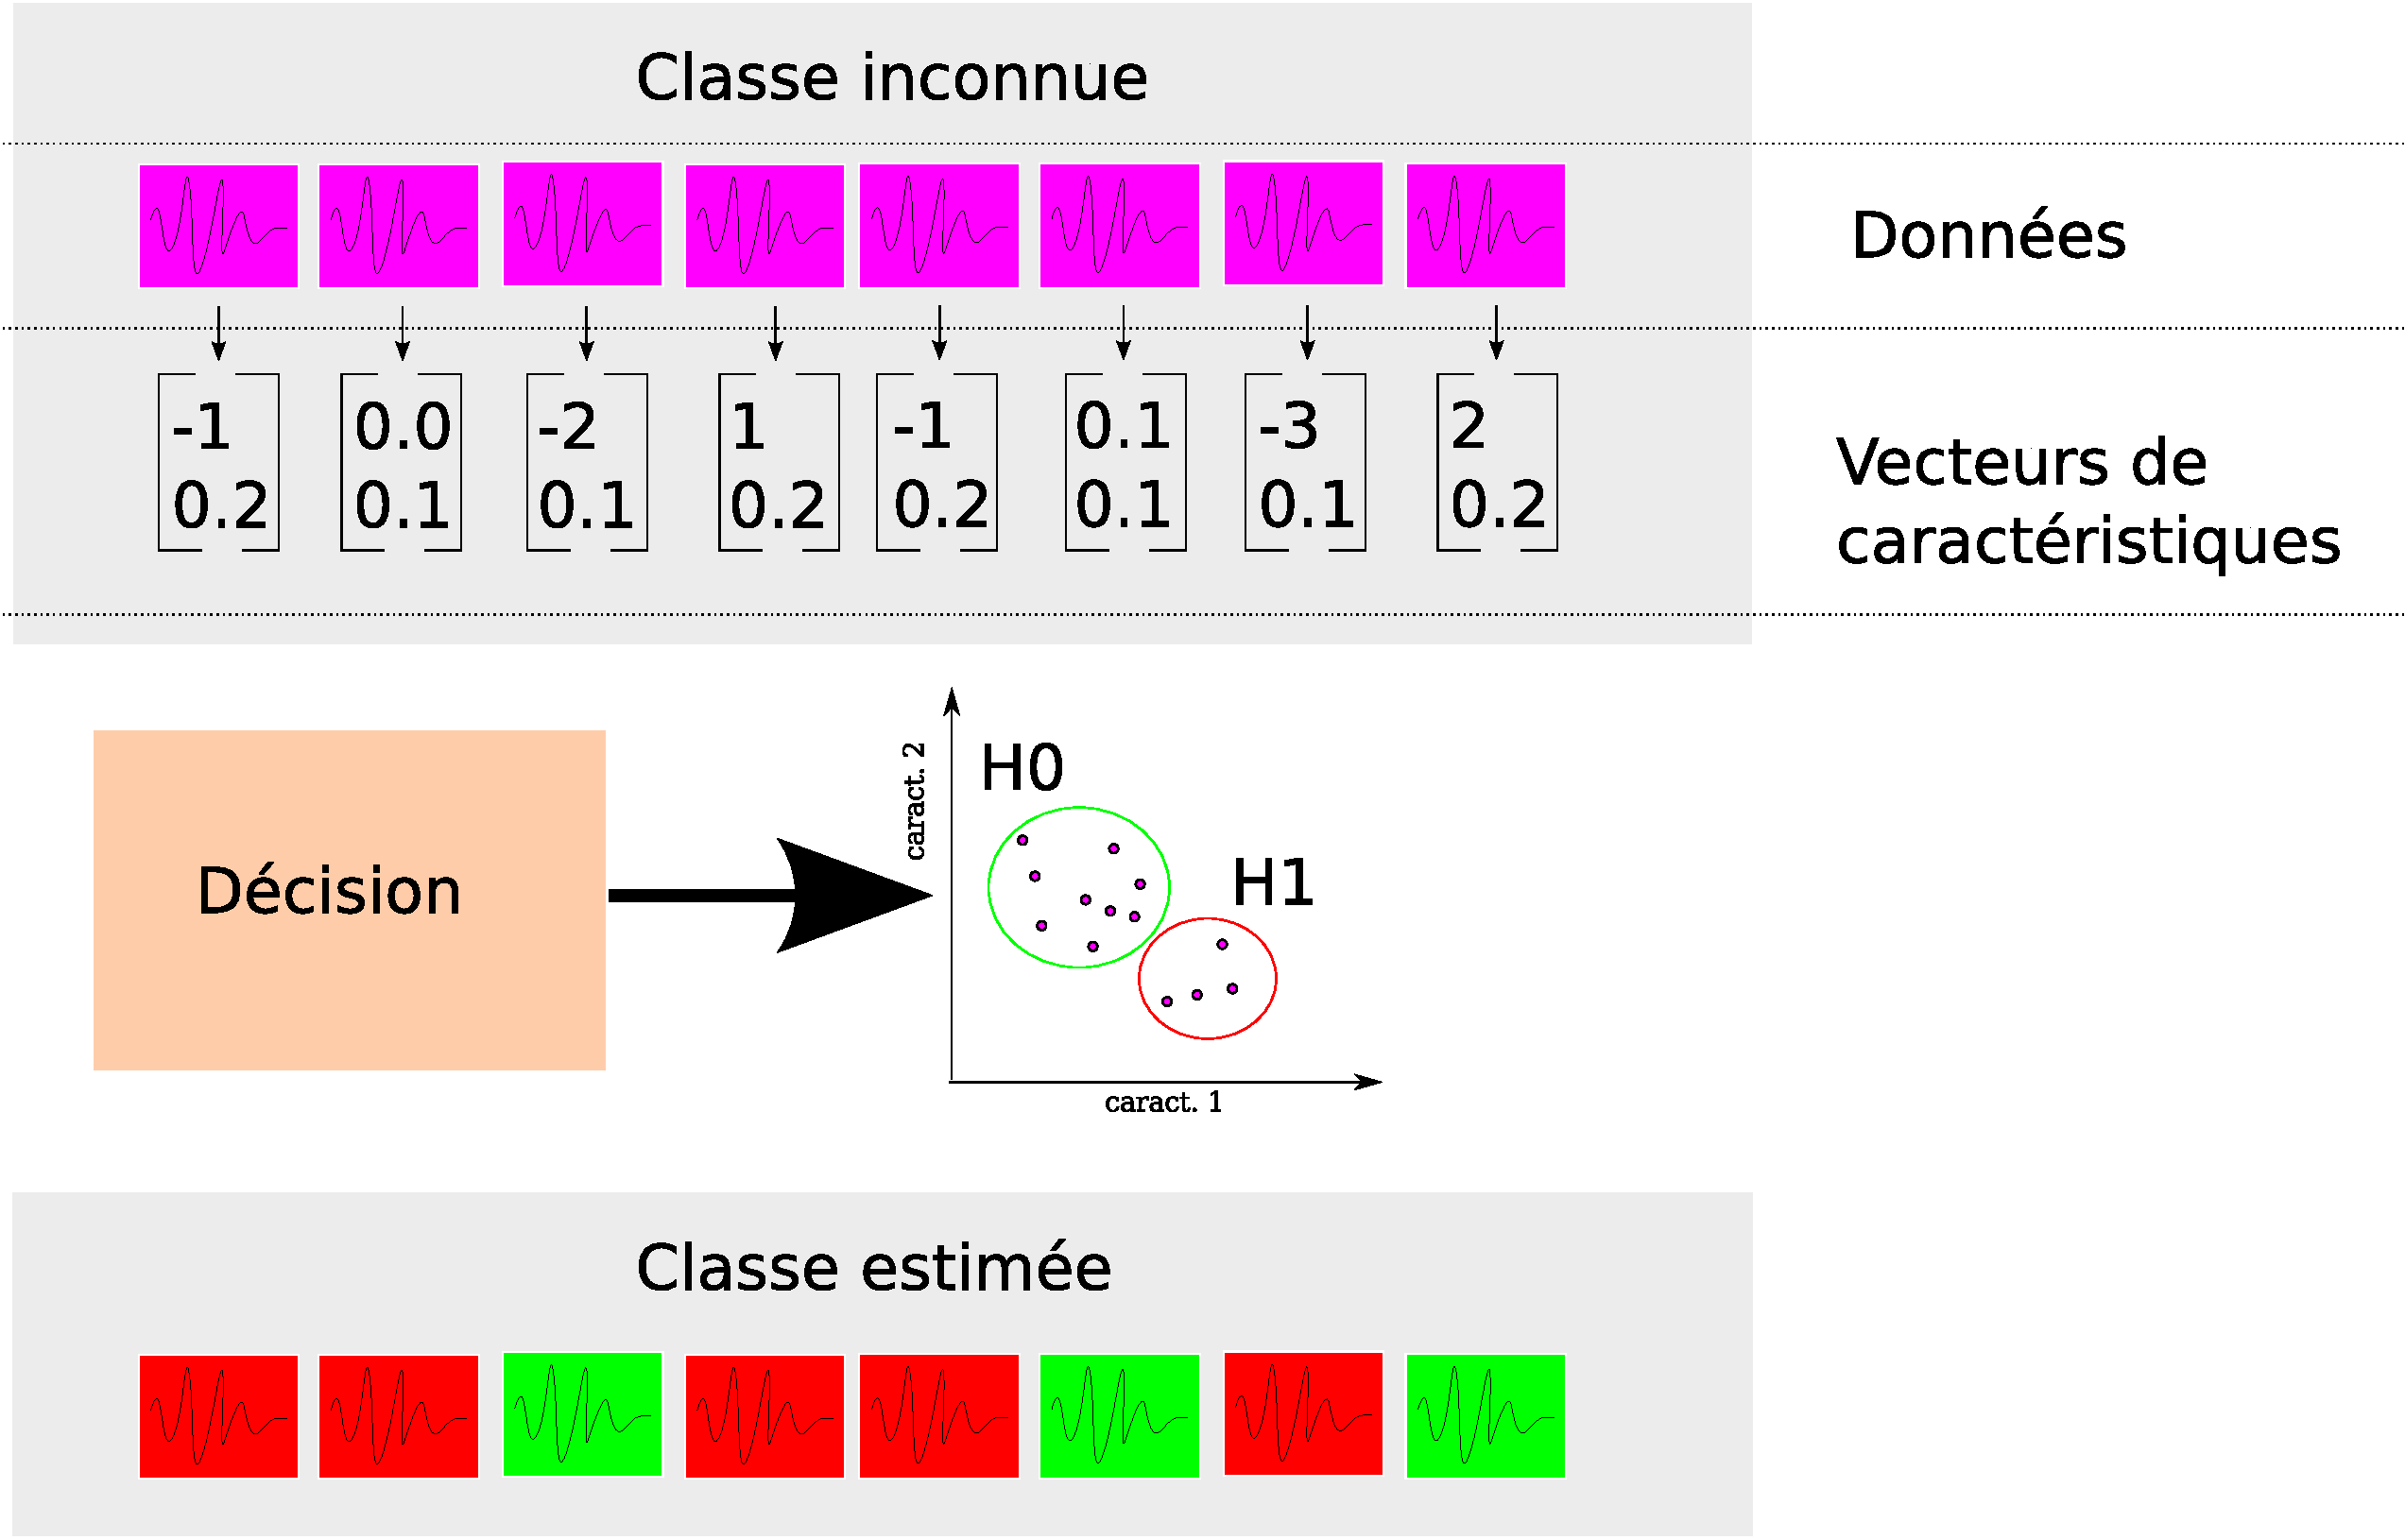
\includegraphics[width=15cm]{images/fonctionnementClassifNonSup}
	\end{center}
	\caption{Fonctionnement d'un classifieur non supervisé : Les données brutes sont envoyées au classifieur qui va les regrouper en classes en fonction de leur répartition dans l'espace des caractéristiques.}
\end{figure}

	\section{classifieurs}

		CROSS-VALIDATION 

		\subsection{SVM (Separateur à Vaste Marge)}

Ce type de classifieur se base sur 

		\subsection{LDA}

	\section{Systèmes humain}
	% besoin d'avoir des données fiables ?